% !TEX program = xelatex
\documentclass[aspectratio=169,11pt]{beamer}

\usepackage{fontspec}
\usepackage{booktabs}
\usepackage{array}
\usepackage{tikz}
\usepackage{graphicx}
\usepackage{xcolor}
\usetikzlibrary{arrows.meta,positioning,fit,backgrounds,calc}

%============================================== fonts
\setsansfont{Segoe UI}
\newfontfamily\bn{Nirmala UI}[Script=Bengali]
\newcommand{\bng}[1]{{\bn #1}}

%============================================== palette
\definecolor{iutblue}{HTML}{1A56A8}
\definecolor{accent}{HTML}{C2452F}
\definecolor{ink}{HTML}{1B2420}
\definecolor{soft}{HTML}{5A6660}
\definecolor{rule}{HTML}{D7DBD8}
\definecolor{good}{HTML}{2F7A4F}
\definecolor{bad}{HTML}{A33326}
\definecolor{panel}{HTML}{F2F5F8}
\definecolor{hl}{HTML}{FFF3CD}

\setbeamercolor{structure}{fg=iutblue}
\setbeamercolor{frametitle}{fg=iutblue,bg=white}
\setbeamercolor{normal text}{fg=ink}
\setbeamercolor{itemize item}{fg=iutblue}
\setbeamercolor{itemize subitem}{fg=soft}
\setbeamerfont{frametitle}{series=\bfseries,size=\Large}
\setbeamertemplate{navigation symbols}{}
\setbeamertemplate{itemize item}{\textbullet}
\setbeamertemplate{itemize subitem}{--}

\setbeamertemplate{footline}{%
  \hbox to\paperwidth{\hfill
  \raisebox{1.6ex}{\color{soft}\scriptsize\insertframenumber\hspace{3mm}}}}

\setbeamertemplate{frametitle}{%
  \vspace{3mm}\hspace{6mm}\usebeamerfont{frametitle}\usebeamercolor[fg]{frametitle}\insertframetitle%
  \vspace{1mm}\\\hspace{6mm}{\color{iutblue}\rule{0.22\paperwidth}{1.1pt}}\vspace{-1mm}}

\newcommand{\eyebrow}[1]{{\scriptsize\color{soft}\MakeUppercase{#1}}\\[1mm]}
\newcommand{\src}[1]{\hfill{\scriptsize\color{soft}#1}}

% compact table settings
\renewcommand{\arraystretch}{1.12}
\newcolumntype{R}{>{\raggedleft\arraybackslash}p{12mm}}

\begin{document}

%================================================================ 1 TITLE
{\setbeamertemplate{footline}{}
\begin{frame}[plain]
\vspace{4mm}
\begin{center}
{\scriptsize\color{soft}DESIGN PROJECT PRESENTATION \; $\cdot$ \; CSE 4610}\\[6mm]
{\LARGE\bfseries\color{iutblue} BenMedHallu}\\[2mm]
{\large\bfseries\color{iutblue} A Fact-Controlled Benchmark for Hallucination\\[1mm] Detection in Bengali Medical Text}\\[7mm]

\begin{tabular}{ccc}
\normalsize Nashat Islam & \normalsize Subha Tamanna Mrittika & \normalsize Atia Zaman\\
{\small\color{soft}220041211} & {\small\color{soft}220041227} & {\small\color{soft}220041241}
\end{tabular}\\[7mm]

{\small\bfseries Under the Supervision of}\\[2mm]
{\normalsize\bfseries Ajwad Abrar Mostofa}\\
{\small Junior Lecturer, Department of Computer Science and Engineering}\\
{\small Islamic University of Technology (IUT), OIC}\\[6mm]
{\small Department of Computer Science and Engineering\\Islamic University of Technology}
\end{center}
\end{frame}}

%================================================================ 2 OVERVIEW
\begin{frame}{Overview}
\vspace{2mm}
\begin{columns}[T]
\begin{column}{0.5\textwidth}
\begin{tabular}{@{}p{7mm}l@{}}
\textbf{01} & Introduction\\[2.2mm]
\textbf{02} & Related Works\\[2.2mm]
\textbf{03} & Methodology\\[2.2mm]
\textbf{04} & Implementation\\[2.2mm]
\textbf{05} & Results\\
\end{tabular}
\end{column}
\begin{column}{0.5\textwidth}
\begin{tabular}{@{}p{7mm}l@{}}
\textbf{06} & Challenges and Limitations\\[2.2mm]
\textbf{07} & Conclusion and Future Direction\\[2.2mm]
\textbf{08} & GitHub and Individual Contribution\\[2.2mm]
\textbf{09} & References\\
\end{tabular}
\end{column}
\end{columns}
\vspace{6mm}
\begin{center}
\colorbox{panel}{\begin{minipage}{0.86\textwidth}\vspace{1mm}
\centering\small
Four task formats \;$\cdot$\; \textbf{17,915} labelled items \;$\cdot$\; \textbf{82,622} detector judgements \;$\cdot$\; six LLMs
\vspace{1mm}\end{minipage}}
\end{center}
\end{frame}

%================================================================ 3 INTRO / PROBLEM
\begin{frame}{Introduction}
\vspace{-1mm}
{\footnotesize
A \textbf{hallucination} in clinical text generation is \textbf{unfaithfulness to a source}, not implausibility. It has two forms: \textbf{extrinsic} -- the output asserts something the source never stated -- and \textbf{intrinsic} -- it asserts something the source contradicts.
\vspace{2mm}

In Bengali medical text both are \textbf{invisible at the surface}. Each of these edits leaves grammatical, register-consistent, confident clinical prose:
\vspace{1mm}
\begin{center}\footnotesize
\begin{tabular}{@{}l@{\hspace{3mm}}c@{\hspace{3mm}}l@{}}
\bng{হিস্টাসিন} & $\longrightarrow$ & \bng{সিটিরিজিন} \hfill{\scriptsize\color{soft}same drug class, different drug}\\
\bng{৫.৯ ইঞ্চি} & $\longrightarrow$ & \bng{৫.৯ ফুট} \hfill{\scriptsize\color{soft}unit rescaled}\\
\bng{রেজাল্ট পজিটিভ} & $\longrightarrow$ & \bng{রেজাল্ট ভালো} \hfill{\scriptsize\color{soft}specific value generalised away}\\
\end{tabular}
\end{center}
\vspace{1mm}
ROUGE and BERTScore are near-invariant to exactly these edits, and the reader most exposed to the error is least equipped to catch it.
}
\vspace{2mm}
\begin{center}
\colorbox{hl}{\begin{minipage}{0.93\textwidth}\vspace{1mm}\footnotesize
\textbf{Problem statement.}\; No resource measures whether LLMs can distinguish faithful Bengali medical text from deliberately corrupted text, and no methodology exists for building one in which the \textbf{gold label}, the \textbf{error type} and the \textbf{item difficulty} are all under the builder's control.
\vspace{1mm}\end{minipage}}
\end{center}
\end{frame}

%================================================================ 4 INTRO / CONTRIBUTIONS
\begin{frame}{Introduction \;--\; Objectives and Contributions}
\vspace{-1mm}
{\small
\textbf{Four challenges specific to this problem:}
\vspace{1mm}
\begin{columns}[T]
\begin{column}{0.5\textwidth}\footnotesize
\textbf{Distribution leakage.} If hallucinated items are machine-written and faithful ones human-written, a detector wins by recognising generated prose.\\[2mm]
\textbf{Label certainty.} An edit meant to remove support may fail silently, mislabelling the item and penalising every detector that answers correctly.
\end{column}
\begin{column}{0.5\textwidth}\footnotesize
\textbf{Register preservation.} Patients repeat details in several forms, so a partial edit leaves the document self-contradicting -- a different phenomenon from the one intended.\\[2mm]
\textbf{Attributable difficulty.} For a score to be diagnostic rather than merely low, only one experimental axis may move at a time.
\end{column}
\end{columns}
\vspace{3.5mm}
\textbf{Contributions:}
\begin{itemize}\setlength\itemsep{0.9mm}\footnotesize
  \item The first hallucination-detection benchmark for Bengali medical text -- \textbf{four task formats, 17,915 labelled items, 82,622 judgements}.
  \item A construction method that \textbf{derives gold labels rather than annotating them}, recording the changed span with every item.
  \item \textbf{Coarsen}, a novel corruption operation isolating \emph{partial} support -- the hardest condition in the benchmark.
  \item An evaluation of six detectors disaggregated by entity type, corruption operation and cost.
  \item A \textbf{generator / detector / judge separation} that keeps the benchmark outside the self-evaluation loop.
\end{itemize}
}
\end{frame}

%================================================================ 5 RW BenHalluEval
\begin{frame}{Related Works \;--\; BenHalluEval}
\vspace{-1mm}
{\small
\eyebrow{Adib, Sani, Esham, Abrar, Tashdeed \& Chowdhury (2026) \;--\; IUT \& UC}
\begin{columns}[T]
\begin{column}{0.56\textwidth}\footnotesize
\textbf{Problem.} No prior work systematically evaluated hallucination in LLMs for Bengali, the sixth most spoken language.\\[1.5mm]
\textbf{Solution.} A four-task framework (QA, code-mixed QA, summarization, mathematical reasoning); 12,000 hallucinated candidates generated with GPT-5.4; nine LLMs evaluated under a \textbf{dual-track protocol}.\\[1.5mm]
\textbf{Results.} BenHalluScore 7.72--55.42\%; three native annotators, Fleiss' $\kappa = 0.911$--$0.926$; CoT prompting helps on 18 of 32 combinations and hurts on 14.
\end{column}
\begin{column}{0.44\textwidth}\footnotesize
\colorbox{panel}{\begin{minipage}{\textwidth}\vspace{1mm}
\textbf{What we adopt}\\[1mm]
The Track A / Track B protocol, and the BanglaCHQ-Summ corpus.\\[2mm]
\textbf{What we invert}\\[1mm]
BenHalluEval corrupts the \textbf{summary} (Fabricated Content, Non-Factual Addition, Direct Contradiction).\\[1mm]
BenMedHallu corrupts the \textbf{source} and never edits the human summary.
\vspace{1mm}\end{minipage}}
\end{column}
\end{columns}
\vspace{2mm}
{\scriptsize\color{soft}Establishes the dual-track baseline for Bengali; BenMedHallu carries it into the clinical domain.}
}
\end{frame}

%================================================================ 6 RW Leave-N-Out
\begin{frame}{Related Works \;--\; Fact-Controlled Diagnosis (Leave-$N$-Out)}
\vspace{-1mm}
{\small
\eyebrow{Suhas BN et al., Interspeech 2025}
\begin{columns}[T]
\begin{column}{0.56\textwidth}\footnotesize
\textbf{Problem.} Benchmarks built by annotating model output cannot say whether detection degrades for one corruption type over another -- type was never a controlled variable.\\[1.5mm]
\textbf{Solution.} Extract atomic facts from a reference, remove $N$ of them from the input, and treat $N$ as an explicit \textbf{difficulty dial} rather than a post-hoc bin. Applied to English clinical dialogue (ACI-Bench).\\[1.5mm]
\textbf{Impact.} Establishes construction-based labelling for clinical summarization, with difficulty controlled by design.
\end{column}
\begin{column}{0.44\textwidth}\footnotesize
\colorbox{panel}{\begin{minipage}{\textwidth}\vspace{1mm}
\textbf{Closest ancestor of this work}\\[1.5mm]
We adopt Leave-$N$-Out directly, with $N \in \{1,2,3\}$.\\[2mm]
\textbf{Two differences}\\[1mm]
ACI-Bench holds \emph{structured English} clinical encounters; our corpus holds \emph{unstructured Bengali} patient messages.\\[1mm]
We add two alteration operations alongside deletion.
\vspace{1mm}\end{minipage}}
\end{column}
\end{columns}
}
\end{frame}

%================================================================ 7 RW MedHallu
\begin{frame}{Related Works \;--\; MedHallu}
\vspace{-1mm}
{\small
\eyebrow{Pandit et al., EMNLP 2025}
\begin{columns}[T]
\begin{column}{0.56\textwidth}\footnotesize
\textbf{Problem.} General-domain hallucination benchmarks understate the risk in medicine, where an error is clinically consequential rather than merely wrong.\\[1.5mm]
\textbf{Solution.} 10,000 medical QA items built on PubMedQA -- \textbf{1,000 human-annotated and 9,000 artificially generated} -- with difficulty-graded hallucinations.\\[1.5mm]
\textbf{Results.} Domain specificity amplifies the impact of hallucination; supplying context before the judgement, and offering a third ``Not Sure'' option, both improve detection.
\end{column}
\begin{column}{0.44\textwidth}\footnotesize
\colorbox{panel}{\begin{minipage}{\textwidth}\vspace{1mm}
\textbf{Methodological sibling}\\[1.5mm]
The same choice we make: \textbf{manufacture} the hallucinations rather than wait for a model to produce them.\\[2mm]
\textbf{Gap it leaves}\\[1mm]
English, journal-derived text, and hallucinations confined to medical terminology -- not the informal, code-mixed patient register we target.
\vspace{1mm}\end{minipage}}
\end{column}
\end{columns}
}
\end{frame}

%================================================================ 8 RW Med-HALT + CMHE
\begin{frame}{Related Works \;--\; Medical hallucination beyond English}
\vspace{-2mm}
{\footnotesize
\begin{columns}[T]
\begin{column}{0.49\textwidth}
\eyebrow{Med-HALT \;--\; Pal et al., CoNLL 2023}
\textbf{Problem.} Hallucination testing had not reached the medical domain.\\[1mm]
\textbf{Solution.} 59k items derived from medical \textbf{examinations} (PubMed, MedMCQA, MedQA-USMLE) across English, Spanish and Chinese, with reasoning and memory-based tests.\\[1mm]
\textbf{Limitation.} Frames hallucination as \emph{incorrect recall} rather than unfaithfulness to a source; remains English-centric.\\[2mm]
{\color{soft}Direct ancestor of our Tracks 2 and 3 -- exam items, and an abstention option.}
\end{column}
\begin{column}{0.49\textwidth}
\eyebrow{CMHE \;--\; Chinese Medical Hallucination Eval, LREC-COLING 2024}
\textbf{Problem.} Medical hallucination evaluation existed only for English.\\[1mm]
\textbf{Solution.} 42k items from Chinese medical dialogue data, with a \textbf{detection / diagnosis / explanation} benchmark; a portion re-verified by medical professionals.\\[1mm]
\textbf{Result.} Establishes that a dedicated, expert-validated medical hallucination benchmark is feasible outside English.\\[2mm]
{\color{bad}\textbf{The gap, stated by someone else:} this exists for Chinese. It does not exist for Bengali.}
\end{column}
\end{columns}
}
\end{frame}

%================================================================ 9 RW positioning
\begin{frame}[shrink=12]{Related Works \;--\; Positioning and Identified Gaps}
\vspace{-1mm}
\begin{center}
{\footnotesize
\begin{tabular}{@{}lllp{34mm}@{}}
\toprule
\textbf{Work} & \textbf{Task} & \textbf{Language} & \textbf{Label provenance}\\
\midrule
TruthfulQA & QA truthfulness & English & Human curation\\
HaluEval & QA, dialogue, summ. & English & Sampling + human filter\\
FactCC & Summarization consistency & English & Rule-based synthesis\\
FActScore & Atomic factual precision & English & Retrieval + LM validation\\
SelfCheckGPT & Detection method & English & Sampling consistency\\
Med-HALT & Medical reasoning & English-centric & Exam-derived\\
MedHallu & Medical QA & English & 1k human + 9k generated\\
CMHE & Medical detection & Chinese & Generated + expert re-check\\
Leave-$N$-Out & Clinical summarization & English & By construction\\
BenHalluEval & Four tasks & Bengali & Generated + 3 annotators\\
BanglaSummEval & Summarization eval. & Bengali & LLM judges\\
\midrule
\textbf{BenMedHallu} & \textbf{Four formats, medical} & \textbf{Bengali} & \textbf{By construction}\\
\bottomrule
\end{tabular}}
\end{center}
\vspace{2mm}
{\footnotesize
\textbf{Linguistic gap} -- medical hallucination benchmarks exist for English and Chinese; the Bengali entries are general-domain.\quad
\textbf{Label-provenance gap} -- annotation-based benchmarks label the errors they encountered, not the errors they designed.\quad
\textbf{Circularity gap} -- where generator, detector and judge share a family, agreement inside that family is indistinguishable from faithfulness.
}
\end{frame}

%================================================================ 10 METHOD inversion
\begin{frame}{Methodology \;--\; The Inversion}
\vspace{-1mm}
{\small
\begin{columns}[T]
\begin{column}{0.48\textwidth}
{\color{bad}\textbf{Conventional construction}}\\[2mm]
\footnotesize
Keep the source fixed, ask a model to rewrite the \textbf{output}, and label the rewrite as hallucinated.\\[2mm]
Consequence: every hallucinated item is machine-written and every faithful item is human-written. The two classes differ in \textbf{fluency, length and idiom} as well as in faithfulness.\\[2mm]
A detector can then score well by recognising \textbf{generated prose} -- without ever checking a fact.
\end{column}
\begin{column}{0.48\textwidth}
{\color{good}\textbf{BenMedHallu}}\\[2mm]
\footnotesize
Take authentic Bengali medical text known to be faithful and apply exactly \textbf{one controlled, recorded edit} that destroys that faithfulness.\\[2mm]
The reference is \textbf{never rewritten}, so faithful and hallucinated items share one text distribution.\\[2mm]
The label is an \textbf{output of the pipeline} rather than a judgement about it, and the record of what changed comes free.
\end{column}
\end{columns}
\vspace{4mm}
\colorbox{panel}{\begin{minipage}{\textwidth}\vspace{1mm}\footnotesize
\textbf{The same inversion runs through all four tracks.}\quad
\textbf{NER} corrupts the sentence around a tagged entity, not the entity label.\quad
\textbf{QA} generates no text at all -- it pairs an untouched question with its real exam distractors.\quad
\textbf{Q-ALT} corrupts the \emph{question}, not the answer.\quad
\textbf{Summarization} corrupts the \emph{source}, not the summary.
\vspace{1mm}\end{minipage}}
}
\end{frame}

%================================================================ 11 METHOD diagram
\begin{frame}{Methodology \;--\; System Pipeline}
\vspace{-2mm}
\begin{center}
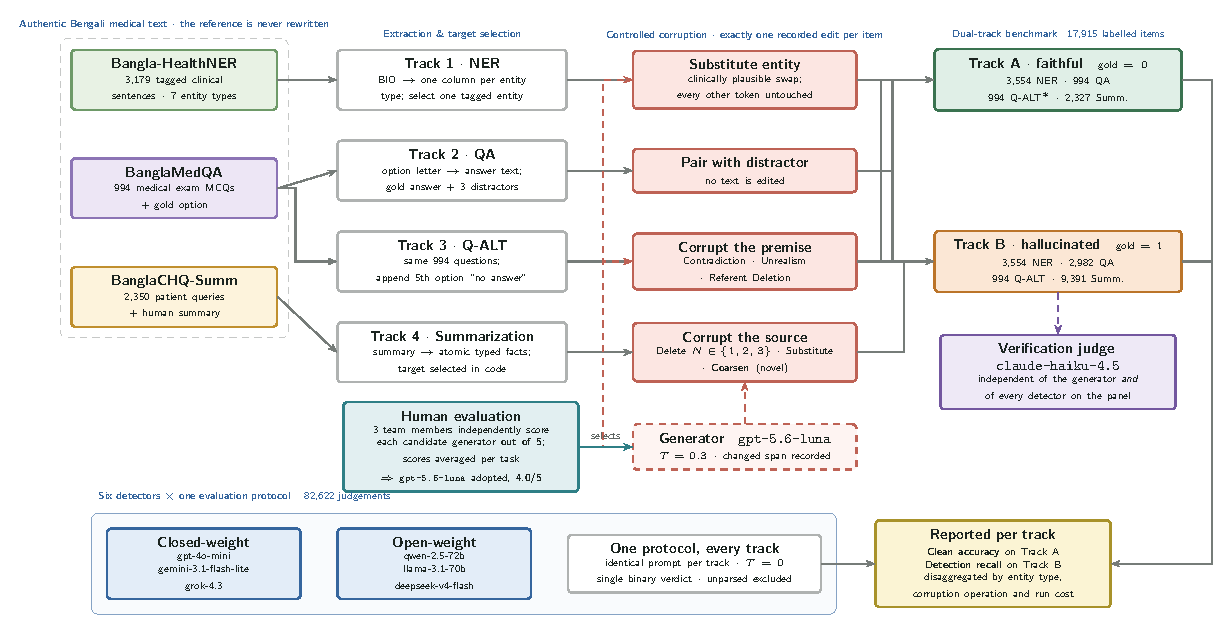
\includegraphics[width=0.985\textwidth]{fig_pipeline.pdf}
\end{center}
\end{frame}

%================================================================ 12 METHOD tracks 1-2
\begin{frame}[shrink=12]{Methodology \;--\; Construction: Tracks 1 and 2}
\vspace{-1mm}
{\footnotesize
\begin{columns}[T]
\begin{column}{0.49\textwidth}
\textbf{Track 1 \;--\; Entity-level (NER)}\\[1.5mm]
\emph{Extraction.} BIO tagging converted to one column per entity type, giving every sentence its tagged clinical entities.\\[1.5mm]
\emph{Selection.} One tagged entity per sentence, chosen in code.\\[1.5mm]
\emph{Generation.} The generator replaces it under four constraints: the replacement must be \textbf{clinically plausible}, \textbf{different} from the original, \textbf{absent elsewhere} in the sentence, and \textbf{every other token untouched}.\\[1.5mm]
\emph{Evaluation.} The detector is shown the sentence and the target entity and returns one binary digit. \textbf{Each row is judged twice} -- clean and corrupted.
\end{column}
\begin{column}{0.49\textwidth}
\textbf{Track 2 \;--\; Answer-level (QA)}\\[1.5mm]
\emph{Extraction.} The gold option letter is resolved to its full answer text.\\[1.5mm]
\emph{Selection.} Each question is paired once with the correct answer and once with each of its \textbf{three real exam distractors}.\\[1.5mm]
\emph{Generation.} \textbf{None.} No text is corrupted -- the distractors were written by the examiners.\\[1.5mm]
\emph{Evaluation.} The detector judges whether the proposed answer is factually correct for the question.\\[1.5mm]
\emph{Why three variants.} They agree within about three points, which shows the ranking is not an artefact of which distractor was drawn.
\end{column}
\end{columns}
}
\end{frame}

%================================================================ 13 METHOD tracks 3-4
\begin{frame}[shrink=12]{Methodology \;--\; Construction: Tracks 3 and 4}
\vspace{-1mm}
{\footnotesize
\begin{columns}[T]
\begin{column}{0.49\textwidth}
\textbf{Track 3 \;--\; Question-level (Q-ALT)}\\[1.5mm]
The same 994 questions, with a fifth option \bng{``উত্তর নেই''} (\emph{no answer}) appended. Each question is rewritten so that \textbf{no option A--D can be correct}, making E the only valid choice. Three techniques:\\[1.5mm]
\emph{Contradiction} -- two individually plausible but jointly impossible premises.\\[1mm]
\emph{Unrealism} -- a clinically styled but factually wrong value or property.\\[1mm]
\emph{Referent Deletion} -- removes the detail behind a confident anaphoric reference whose antecedent was never supplied.\\[1.5mm]
Only selecting the fifth option counts as detection.
\end{column}
\begin{column}{0.49\textwidth}
\textbf{Track 4 \;--\; Document-level (Summarization)}\\[1.5mm]
\emph{Stage 1 -- Extraction.} The human summary is decomposed into \textbf{atomic typed facts} across ten clinical categories.\\[1.5mm]
\emph{Stage 2 -- Selection.} A \textbf{seeded RNG selects the target in code}, not the model. This preserves the gold record, the category balance and the difficulty dial, and makes reruns reproducible.\\[1.5mm]
\emph{Stage 3 -- Generation.} The source is rewritten so the target loses support while every retained fact survives. Three operations: \textbf{Delete} $N\!\in\!\{1,2,3\}$, \textbf{Substitute}, \textbf{Coarsen}.\\[1.5mm]
\emph{Stage 4 -- Verification.} An independent judge checks each fact before acceptance.
\end{column}
\end{columns}
\vspace{2mm}
\colorbox{panel}{\begin{minipage}{\textwidth}\vspace{.8mm}
\textbf{Three support relations, by design.}\;
\textbf{Delete} leaves the claim \emph{unsupported} (extrinsic).\;
\textbf{Substitute} leaves it \emph{contradicted} (intrinsic).\;
\textbf{Coarsen} replaces a specific value with a vaguer one still true of the original -- \emph{partial} support.
\vspace{.8mm}\end{minipage}}
}
\end{frame}

%================================================================ 14 METHOD protocol
\begin{frame}[shrink=12]{Methodology \;--\; Selection and Protocol}
\vspace{-1mm}
{\footnotesize
\textbf{Generator selection was measured, not assumed.}\\[1.5mm]
A pilot study scored the candidates two ways: \textbf{three team members independently rated each generator's output out of five} per task, averaged below; and an automated bake-off scored the same items with independent judges, where a \emph{lower} detection rate indicates harder items.
\vspace{2mm}
\begin{center}{\scriptsize
\begin{tabular}{@{}lccccc@{}}
\toprule
\textbf{Candidate generator} & \textbf{Medicine} & \textbf{Symptom} & \textbf{Health Cond.} & \textbf{Summarization} & \textbf{Mean}\\
\midrule
\textbf{gpt-5.6-luna} & \textbf{4.0} & \textbf{4.0} & \textbf{4.0} & \textbf{4.0} & \textbf{4.00}\\
deepseek-v4-pro & 4.0 & 4.0 & 3.5 & 3.0 & 3.63\\
claude-opus-5 & 3.0 & 4.0 & -- & -- & 3.50\\
qwen-3.8-max & 3.5 & 3.0 & -- & -- & 3.25\\
\bottomrule
\end{tabular}}\\[1mm]
{\scriptsize\color{soft}Mean human rating out of 5 over three independent reviewers. \texttt{gpt-5.6-luna} was best or tied on every task and was adopted as the sole generator.}
\end{center}
\vspace{1.5mm}
\textbf{One protocol for every track.}\;
An identical prompt per track is issued to all six detectors at $T=0$; each returns a single binary verdict; unparseable verdicts are \textbf{excluded from the denominator} rather than defaulted.
\vspace{1mm}

\textbf{Anti-circularity.}\;
Generator, detectors and judge come from \textbf{disjoint model families}; a panel member is never the judge, so family agreement cannot be mistaken for faithfulness.
}
\end{frame}

%================================================================ 15 IMPLEMENTATION
\begin{frame}[shrink=12]{Implementation}
\vspace{-1mm}
{\footnotesize
\begin{columns}[T]
\begin{column}{0.5\textwidth}
\textbf{Source corpora}\\[1mm]
\begin{tabular}{@{}p{22mm}p{32mm}@{}}
\textbf{Bangla-HealthNER} & Khan et al., \emph{NERvous About My Health}, EMNLP Findings 2023 -- 3,179 tagged clinical sentences\\[1.5mm]
\textbf{BanglaCHQ-Summ} & Khan et al., ACL 2023 -- 2,350 patient queries with human summaries\\[1.5mm]
\textbf{bangla-med-qa} & 994 medical examination MCQs with gold options\\
\end{tabular}
\vspace{2.5mm}
\textbf{Architecture}\\[1mm]
A four-stage repository: \texttt{preprocessing/} holds the generation pipelines, \texttt{dataset/} the assembled benchmark, \texttt{evaluation\_*/} the detector runs, and aggregation scripts produce the reported tables. Prompts and selection logic live in \textbf{importable modules, not notebooks}, so each prompt exists in exactly one place.
\end{column}
\begin{column}{0.48\textwidth}
\textbf{Models}\; -- all eight reached through OpenRouter, giving one client, one retry policy and one cost ledger across six vendors.\\[1mm]
\begin{tabular}{@{}ll@{}}
Generator & \texttt{gpt-5.6-luna}\\
Judge & \texttt{claude-haiku-4.5}\\
Detectors & \texttt{gpt-4o-mini}\\
 & \texttt{gemini-3.1-flash-lite}\\
 & \texttt{grok-4.3}\\
 & \texttt{qwen-2.5-72b-instruct}\\
 & \texttt{llama-3.1-70b-instruct}\\
 & \texttt{deepseek-v4-flash}\\
\end{tabular}
\vspace{2.5mm}
\textbf{Reliability at scale}\\[1mm]
Runs against six commercial APIs at tens of thousands of calls fail constantly. Results are \textbf{checkpointed every fifty rows} and every run resumes from its own output file; multiple API keys rotate on HTTP 402 and 429; a repair pass re-runs only rows whose verdict is null; and a \textbf{pre-flight probe} issues one call per detector before committing a full run.
\end{column}
\end{columns}
}
\end{frame}

%================================================================ 16 RESULTS inventory + T1
\begin{frame}[shrink=12]{Results \;--\; Benchmark Inventory and Track 1}
\vspace{-2mm}
{\footnotesize
\begin{columns}[T]
\begin{column}{0.36\textwidth}
\textbf{Benchmark inventory}\\[1mm]
\begin{tabular}{@{}lrr@{}}
\toprule
\textbf{Track} & \textbf{Items} & \textbf{Judg.}\\
\midrule
NER & 3,554 & 38,540\\
QA & 3,976 & 23,856\\
Q-ALT & 994 & 5,964\\
Summarization & 9,391 & 14,262\\
\midrule
\textbf{Total} & \textbf{17,915} & \textbf{82,622}\\
\bottomrule
\end{tabular}\\[3mm]
{\scriptsize Judgement counts reflect \emph{actual} detector coverage rather than the nominal six models.}\\[3mm]
{\scriptsize\color{soft}\textbf{Clean accuracy} -- accuracy on the faithful member of a pair.\\[1mm]
\textbf{Recall} -- proportion of corrupted items correctly flagged.\\[1mm] The gap between them is the principal finding.}
\end{column}
\begin{column}{0.62\textwidth}
\textbf{Track 1 -- detection recall (\%) by entity type}\\[1mm]
\begin{tabular}{@{}lrrrrrr@{}}
\toprule
\textbf{Detector} & \textbf{Med.} & \textbf{Age} & \textbf{Dos.} & \textbf{H.C.} & \textbf{Spec.} & \textbf{Proc.}\\
\midrule
Grok-4.3 & \textbf{94.7} & -- & -- & \textbf{69.2} & \textbf{83.5} & \textbf{73.6}\\
DeepSeek V4 Flash & 79.6 & 96.6 & 83.0 & 68.5 & 80.2 & 51.2\\
Gemini 3.1 fl.-lite & 75.3 & -- & \textbf{87.3} & 57.0 & 64.9 & 62.0\\
GPT-4o-mini & 73.3 & 94.7 & 82.2 & 61.7 & 64.6 & 53.7\\
Qwen 2.5 72B & 69.9 & \textbf{99.6} & 81.0 & 67.9 & 72.3 & 55.8\\
Llama 3.1 70B & 54.4 & 73.1 & -- & 22.7 & 15.9 & 31.8\\
\bottomrule
\end{tabular}\\[1mm]
{\scriptsize A dash marks a detector not run on that category.}\\[2.5mm]
{\scriptsize
\textbf{Entity type strongly predicts difficulty.} Age and Dosage are close to solved (73--99.6\%): the corrupted value is a \emph{number}, and a number mismatching its context is easy to spot. Health Condition, Specialist and Medical Procedure require \emph{clinical knowledge} rather than pattern matching, and every detector falls away.\\[1.5mm]
\textbf{The Llama row.} At 15.9\% on Specialist it accepts five of six swapped entities while scoring 93.9\% on the matching clean sentences -- agreeing with the prompt rather than reading the pair.}
\end{column}
\end{columns}
}
\end{frame}

%================================================================ 17 RESULTS T2 T3
\begin{frame}[shrink=12]{Results \;--\; Tracks 2 and 3}
\vspace{-2mm}
{\footnotesize
\begin{columns}[T]
\begin{column}{0.46\textwidth}
\textbf{Track 2 -- answer-level (\%)}\\[1mm]
\begin{tabular}{@{}lrr@{}}
\toprule
\textbf{Detector} & \textbf{Accepts correct} & \textbf{Rejects wrong}\\
\midrule
Grok-4.3 & \textbf{86.3} & \textbf{92.2}\\
Gemini 3.1 flash-lite & 86.1 & 90.0\\
DeepSeek V4 Flash & 81.0 & 89.6\\
GPT-4o-mini & 66.9 & 84.7\\
Qwen 2.5 72B & 67.2 & 78.2\\
Llama 3.1 70B & 71.1 & 70.8\\
\bottomrule
\end{tabular}\\[2mm]
{\scriptsize Wrong-answer recall is the mean over three distractor variants, which agree within about three points.}\\[2.5mm]
{\scriptsize\textbf{The bias direction reverses relative to Track 1.} There, models \emph{under}-flag and accept corrupted text. Here they \emph{over}-flag: GPT-4o-mini rejects a third of the medically correct answers while still catching 84.7\% of the wrong ones. One model carries two opposite failure modes depending on framing -- the clearest evidence for building four task formats rather than one.}
\end{column}
\begin{column}{0.52\textwidth}
\textbf{Track 3 -- question-level, detection rate (\%)}\\[1mm]
\begin{tabular}{@{}lrrrr@{}}
\toprule
\textbf{Detector} & \textbf{Contra.} & \textbf{Unreal.} & \textbf{Ref. Del.} & \textbf{Overall}\\
\midrule
Grok-4.3 & \textbf{95.0} & \textbf{91.9} & \textbf{82.6} & \textbf{88.8}\\
DeepSeek V4 Flash & 72.0 & 76.7 & 47.0 & 60.6\\
Gemini 3.1 fl.-lite & 62.4 & 62.8 & 46.4 & 54.8\\
GPT-4o-mini & 46.1 & 58.1 & 53.8 & 50.8\\
Qwen 2.5 72B & 51.8 & 47.7 & 37.9 & 44.9\\
\bottomrule
\end{tabular}\\[1mm]
{\scriptsize Items: Contradiction 436, Referent Deletion 472, Unrealism 86. Llama 3.1 70B is excluded -- its run stalled after 211 of 994 items.}\\[2.5mm]
{\scriptsize\textbf{The hardest track in the benchmark}, and technique matters as much as model. \textbf{Referent Deletion} is hardest for four of five detectors, and by a wide margin -- DeepSeek drops from 72.0\% to 47.0\%.\\[1.5mm]
The reason is structural: Contradiction and Unrealism both insert something \emph{false}, which clinical knowledge can catch. Referent Deletion inserts nothing false at all -- it \emph{removes} something, leaving a confident reference with no antecedent.}
\end{column}
\end{columns}
}
\end{frame}

%================================================================ 18 RESULTS T4
\begin{frame}[shrink=12]{Results \;--\; Track 4 and the Operation Gradient}
\vspace{-2mm}
{\footnotesize
\begin{columns}[T]
\begin{column}{0.41\textwidth}
\textbf{Track 4 -- overall (\%) and run cost}\\[1mm]
{\scriptsize
\begin{tabular}{@{}l@{\hspace{1.4mm}}r@{\hspace{1.4mm}}r@{\hspace{1.4mm}}r@{\hspace{1.4mm}}r@{}}
\toprule
\textbf{Detector} & \textbf{Cln.} & \textbf{Cor.} & \textbf{Ovr.} & \textbf{USD}\\
\midrule
Grok-4.3 & 89.1 & \textbf{94.2} & \textbf{93.2} & 4.567\\
Gemini 3.1 fl.-lite & 89.3 & 93.5 & 92.6 & \textbf{0.137}\\
Qwen 2.5 72B & 89.6 & 87.8 & 88.1 & 0.489\\
GPT-4o-mini & \textbf{93.6} & 78.0 & 81.1 & 0.098\\
Llama 3.1 70B & 78.0 & 81.1 & 80.5 & 0.697\\
DeepSeek V4 Flash & 89.6 & 72.9 & 76.2 & 0.121\\
\bottomrule
\end{tabular}}\\[3mm]
{\scriptsize\textbf{Scale and price are weak predictors.} Grok-4.3 finishes first at 93.2\% but costs \textbf{\$4.57} against \textbf{\$0.137} for Gemini 3.1 flash-lite, which finishes \textbf{0.58 points behind} -- a thirty-three-fold cost difference for a gap well inside single-run noise.\\[2mm]
GPT-4o-mini again inverts its Track 1 profile: best of all six on untouched pairs at 93.6\%, but only 78.0\% on corrupted sources.}
\end{column}
\begin{column}{0.57\textwidth}
\textbf{Recall (\%) by corruption operation}\\[1mm]
{\scriptsize
\begin{tabular}{@{}l@{\hspace{1.4mm}}r@{\hspace{1.4mm}}r@{\hspace{1.4mm}}r@{\hspace{1.4mm}}r@{\hspace{1.4mm}}r@{}}
\toprule
\textbf{Detector} & \textbf{Del.1} & \textbf{Del.2} & \textbf{Del.3} & \textbf{Subst.} & \textbf{Coars.}\\
\midrule
Grok-4.3 & 98.0 & 100.0 & 100.0 & \textbf{95.9} & \textbf{72.7}\\
Gemini 3.1 fl.-lite & 97.4 & 100.0 & 100.0 & 94.0 & 71.7\\
Qwen 2.5 72B & 90.6 & 99.2 & 99.7 & 84.3 & 62.3\\
Llama 3.1 70B & 85.3 & 92.1 & 96.0 & 72.2 & 59.3\\
DeepSeek V4 Flash & 70.9 & 82.8 & 84.8 & 73.1 & 51.2\\
GPT-4o-mini & 77.6 & 91.3 & 93.3 & 80.2 & 42.7\\
\midrule
\textbf{Mean} & \textbf{86.6} & \textbf{94.2} & \textbf{95.6} & \textbf{83.3} & \textbf{60.0}\\
\bottomrule
\end{tabular}}\\[3mm]
{\scriptsize\textbf{Two clean gradients.}\\[1.5mm]
\textbf{(1) Deletion becomes easier as $N$ rises}, from 86.6\% at one fact to 95.6\% at three. More missing material means more signal, and the trend holds across \emph{all six} detectors -- confirming $N$ works as the intended difficulty dial.\\[1.5mm]
\textbf{(2) Coarsen collapses.} At a mean of 60.0\% it sits 23 points below Substitute and 36 below three-fact deletion; GPT-4o-mini catches only 42.7\%. The source still discusses the detail and points the same way, so a detector checking \emph{topical agreement} finds it and stops.}\vspace{-2mm}
\end{column}
\end{columns}
}
\end{frame}

%================================================================ 19 RESULTS qualitative
\begin{frame}[shrink=12]{Results \;--\; Qualitative Samples Across All Four Tracks}
\vspace{-3mm}
{\scriptsize\color{soft}Bold figures give how many detectors correctly flagged the item. Samples span the difficulty range.}\\[1.5mm]
{\scriptsize
\begin{columns}[T]
\begin{column}{0.49\textwidth}
\textbf{Track 1 -- NER}\\[1mm]
\colorbox{panel}{\begin{minipage}{0.96\textwidth}\vspace{.7mm}
\emph{Medicine}\; \bng{হিস্টাসিন} $\rightarrow$ \bng{সিটিরিজিন} \hfill \textbf{3/6}\\
{\color{soft}Same drug class, different drug.}\\[1.2mm]
\emph{Specialist}\; ``Heart er doctors'' $\rightarrow$ ``Pulmonologist'' \hfill \textbf{3/6}\\
{\color{soft}Cardiologist to pulmonologist.}\\[1.2mm]
\emph{Health Cond.}\; \bng{বদহজম} $\rightarrow$ \bng{গ্যাস্ট্রাইটিস} \hfill \textbf{3/6}\\
{\color{soft}An adjacent diagnosis, not the same one.}
\vspace{.7mm}\end{minipage}}\\[1.8mm]
\textbf{Track 2 -- QA}\\[1mm]
\colorbox{panel}{\begin{minipage}{0.96\textwidth}\vspace{.7mm}
\bng{মাথার খুলিতে কয়টি হাড় রয়েছে?} \hfill \textbf{3/6}\\
{\color{soft}Proposed answer \textbf{23}; three of six accepted it.}
\vspace{.7mm}\end{minipage}}\\[1.8mm]
\textbf{Track 3 -- Q-ALT}\\[1mm]
\colorbox{panel}{\begin{minipage}{0.96\textwidth}\vspace{.7mm}
\emph{Contradiction} \hfill \textbf{2/5}\\
{\color{soft}The deltoid tuberosity placed on \emph{both} the scapula and the humerus -- anatomically impossible.}
\vspace{.7mm}\end{minipage}}
\end{column}
\begin{column}{0.49\textwidth}
\textbf{Track 4 -- Summarization}\\[1mm]
\colorbox{panel}{\begin{minipage}{0.96\textwidth}\vspace{.7mm}
\emph{Coarsen} \hfill \textbf{0/6}\\
\bng{রেজাল্ট পজিটিভ আসছে} $\rightarrow$ \bng{রেজাল্ট ভালো আসছে}\\
summary claims \bng{প্রেগ্ন্যাসি টেস্ট পজিটিভ}\\
{\color{soft}``Came out good'' no longer supports ``positive''.}
\vspace{.7mm}\end{minipage}}\\[1.8mm]
\colorbox{panel}{\begin{minipage}{0.96\textwidth}\vspace{.7mm}
\emph{Substitute} \hfill \textbf{0/6}\\
\bng{শ্বাসকষ্ট হয় কিছুটা} $\rightarrow$ \bng{মাথা ঘোরে কিছুটা}\\
summary claims \bng{শ্বাসকষ্ট হয় কিছুটা}\\
{\color{soft}Breathing difficulty became dizziness.}
\vspace{.7mm}\end{minipage}}\\[1.8mm]
\colorbox{panel}{\begin{minipage}{0.96\textwidth}\vspace{.7mm}
\emph{Delete} $N\!=\!1$ \hfill \textbf{2/6}\\
{\color{soft}87 characters removed, including the whole account of the 14-day antibiotic course healing the fissure -- yet the summary still claims it healed.}
\vspace{.7mm}\end{minipage}}
\end{column}
\end{columns}
}
\end{frame}

%================================================================ 20 CHALLENGES
\begin{frame}[shrink=12]{Challenges and Limitations}
\vspace{-2mm}
{\footnotesize
\begin{columns}[T]
\begin{column}{0.49\textwidth}
\textbf{Challenges}\\[1.5mm]
\textbf{Inconsistent verdict polarity.} The NER prompts were developed in two groups with opposite conventions -- for some categories a verdict of 1 means \emph{supported}, for others \emph{hallucinated}. Applying one convention uniformly silently inverts half the results rather than producing an obvious error.\\[1.5mm]
\textbf{API reliability at scale.} Credit exhaustion and rate limiting interrupted long runs constantly. Key rotation, checkpointing and repair passes recovered most but not all: the Llama Q-ALT run stalled at 211 of 994 items.\\[1.5mm]
\textbf{Reasoning models returning empty completions.} A model whose reasoning budget exceeds the token cap returns an empty string rather than an error -- discovered only after a batch had been spent, which led to the mandatory pre-flight probe.\\[1.5mm]
\textbf{Cost control.} One frontier detector cost \$4.57 on a single track against \$0.10--\$0.14 for flash-tier models, forcing a decision about which tracks the expensive models could cover.
\end{column}
\begin{column}{0.49\textwidth}
\textbf{Limitations}\\[1.5mm]
\textbf{Verification not applied to the released set.} The judge is implemented but was not run over the assembled dataset within the timeline, so released items passed only the two mechanical filters. A residual proportion may carry an incorrect gold label, which would depress all six detectors' recall roughly equally -- the reported \textbf{rankings are therefore more trustworthy than the absolute values}.\\[1.5mm]
\textbf{Coverage.} Symptom, the largest entity type, reached generation only. Age and Dosage were evaluated by four detectors rather than six. The Llama Q-ALT run is incomplete, and 7,483 corrupted summarization items in the training split remain unscored.\\[1.5mm]
\textbf{No clinical validation.} All corruptions are model-generated; no clinician has confirmed the substituted entities are plausible in context.\\[1.5mm]
\textbf{Statistical treatment.} A single prompt at temperature 0, with no prompt-sensitivity study or significance testing. Differences of one or two points should not be treated as meaningful.
\end{column}
\end{columns}
}
\end{frame}

%================================================================ 21 CONCLUSION
\begin{frame}[shrink=12]{Conclusion and Future Direction}
\vspace{-2mm}
{\footnotesize
\textbf{The central result is a gap, not an average.}\;
Six contemporary models read faithful Bengali medical text almost perfectly and miss between 5\% and 84\% of the corruptions inserted into it. That gap widens systematically as the corruption becomes \emph{less like an error and more like an omission}.
\vspace{2mm}
\begin{columns}[T]
\begin{column}{0.5\textwidth}
\textbf{Findings against the research questions}\\[1.5mm]
\textbf{RQ1} -- affirmatively but narrowly: frontier models can detect Bengali medical hallucination, but only Grok-4.3 does so reliably on \emph{both} halves of a pair.\\[1.2mm]
\textbf{RQ2} -- entity type strongly predicts difficulty: numeric types reach 73--99.6\%, types requiring clinical knowledge fall to 15.9--86.4\%.\\[1.2mm]
\textbf{RQ3} -- the operation matters more than the entity type, with mean recall spanning 36 points from Coarsen (60.0\%) to three-fact deletion (95.6\%).\\[1.2mm]
\textbf{RQ4} -- negatively: a 70B open-weight model places last on every track it completed, and a flash-tier model matches a frontier reasoning model within 0.6 points at one thirty-third the cost.
\end{column}
\begin{column}{0.48\textwidth}
\textbf{Future work}\\[1.5mm]
\textbf{1. Run the verification judge.} Stage 4 is written and parked; executing it converts a well-filtered dataset into a verified one.\\[1.2mm]
\textbf{2. Close the coverage gaps.} Score the Symptom track, add the missing detectors to Age and Dosage, rerun Llama, and score the unevaluated summarization split.\\[1.2mm]
\textbf{3. Score span localisation}, which needs no new data -- every item already stores the original and replacement spans.\\[1.2mm]
\textbf{4. Human clinical validation} of a stratified sample by Bangladeshi clinicians.\\[1.2mm]
\textbf{5. Cheap supervised baselines.} With the benchmark in place, fine-tuning BanglaBERT tests whether a small supervised model can approach a commercial API.\\[1.2mm]
\textbf{6. Other low-resource languages.} The pipeline is language-agnostic apart from its prompts.
\end{column}
\end{columns}
\vspace{2mm}
\centering\colorbox{hl}{\begin{minipage}{0.93\textwidth}\vspace{1mm}
\centering Coarsening a value rather than falsifying it defeats every detector tested, and no existing benchmark isolates that condition.
\vspace{1mm}\end{minipage}}
}
\end{frame}

%================================================================ 22 GITHUB + CONTRIB
\begin{frame}{GitHub and Individual Contribution}
\vspace{-1mm}
{\footnotesize
\begin{center}
\textbf{Repository}\; \texttt{https://github.com/nashatislam/benmedhallu-priv}
\end{center}
\vspace{3mm}
\begin{center}
\begin{tabular}{@{}p{34mm}p{34mm}p{34mm}@{}}
\toprule
\textbf{Nashat Islam}\newline{\scriptsize 220041211} &
\textbf{Subha Tamanna Mrittika}\newline{\scriptsize 220041227} &
\textbf{Atia Zaman}\newline{\scriptsize 220041241}\\
\midrule
{\scriptsize $\bullet$ Track 1 (NER) generation and evaluation pipelines}\newline
{\scriptsize $\bullet$ Track 2 (QA) construction and detector runs}\newline
{\scriptsize $\bullet$ Repository architecture and cost ledger}\newline
{\scriptsize $\bullet$ Human evaluation reviewer} &
{\scriptsize $\bullet$ Track 4 (Summarization) source-corruption pipeline}\newline
{\scriptsize $\bullet$ Fact extraction and Coarsen operation design}\newline
{\scriptsize $\bullet$ Verification judge implementation}\newline
{\scriptsize $\bullet$ Human evaluation reviewer} &
{\scriptsize $\bullet$ Track 3 (Q-ALT) technique design and generation}\newline
{\scriptsize $\bullet$ NER category expansion and evaluation}\newline
{\scriptsize $\bullet$ Results aggregation and reporting tables}\newline
{\scriptsize $\bullet$ Human evaluation reviewer}\\
\bottomrule
\end{tabular}
\end{center}
\vspace{4mm}
\begin{center}{\color{soft}\scriptsize Literature survey, benchmark design decisions, pilot generator selection and the final report were carried out jointly.}\end{center}
}
\end{frame}

%================================================================ 23 THANKS
{\setbeamertemplate{footline}{}
\begin{frame}[plain]
\vspace{22mm}
\begin{center}
{\Huge\bfseries\color{iutblue} Thank You}
\end{center}
\end{frame}}

\end{document}
